\section{Descargas}
El siguiente proyecto con sus respectivos archivos se encuentra para ser descargado en el repositorio GitHub.
\begin{figure}[htb]
	\centering
	
\includegraphics[scale=0.5]{gitTunel.png}
	\captionof{figure}{Repositorio en Github}
	\label{fig:git}
\end{figure}

\url{https://github.com/UNPSJB-YC/Automatizacion_Tunel_UNPSJB}
\newpage








\begin{center}
	{
\includegraphics[width=0.2\textwidth]{unpsjb.png}\par}
	\vspace{1cm}
	{\bfseries\LARGE Universidad Nacional de la Patagonia\\ San Juan Bosco \par}
	\vspace{1cm}
	{\scshape\Large Facultad de Ingenier\'ia \par}
	\vspace{3cm}
	{\scshape\Huge Automatización de Túnel de Viento \par}
	{\itshape\Large -ESQUEMÁTICOS DE LAS PLACAS- \par}
	
	
	\vspace{3cm}
	{\itshape\Large Proyecto Final de Carrera\\ - Ingeniería Electrónica - \par}
	\vfill
	{\Large Autores: \par}
	{\Large Caamiña Quineros, Daniela Beatriz\\ Yapura, Cristian Alejandro \par}
	\vfill
	{\Large Diciembre 2021 \par}
\end{center}





\newpage



\section{Esquemático de la placa implementada}
\begin{figure}[H]
	\centering
	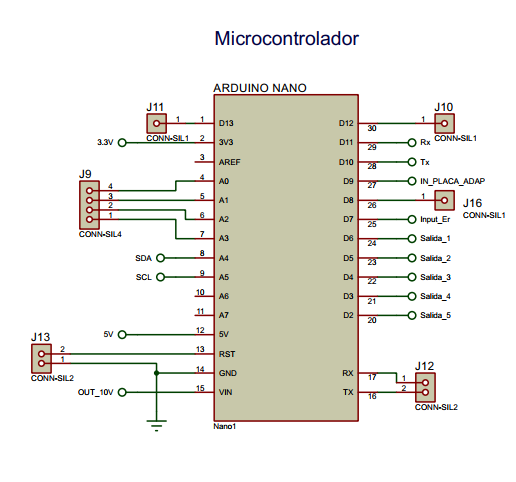
\includegraphics[scale=1]{A_Placa_2.png}
	\captionof{figure}{Esquema del microcontrolador}
\end{figure}
\begin{figure}[H]
	\centering	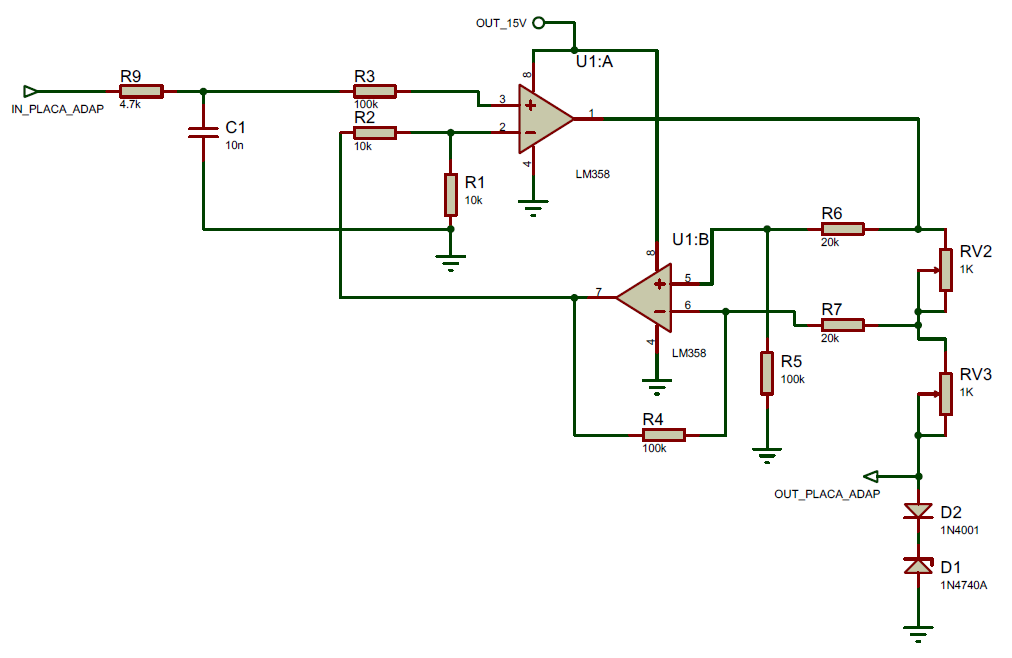
\includegraphics[scale=0.8,angle =90]{A_Placa_1.png}
	\captionof{figure}{Esquema de la placa adaptadora de la señal del sensor de presión diferencial.}
\end{figure}
\begin{figure}[H]
	\centering
	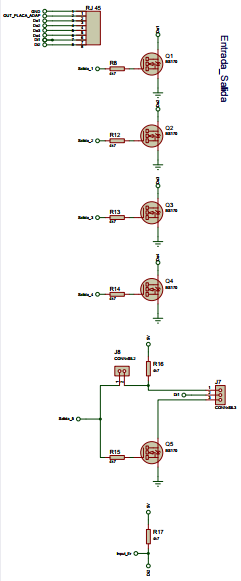
\includegraphics[scale=0.5]{A_Placa_3.png}
	
	\caption{Esquema de entradas y salidas del microcontrolador hacia el variador.} 
\end{figure}
\begin{figure}[H]
	\centering	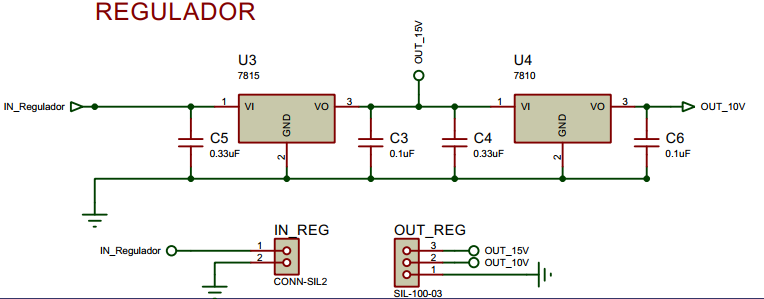
\includegraphics[scale=0.8]{A_Placa_4.png}
\end{figure}	
\captionof{figure}{Esquema de la placa reguladora de tensión.}
\begin{figure}[H]
	\centering	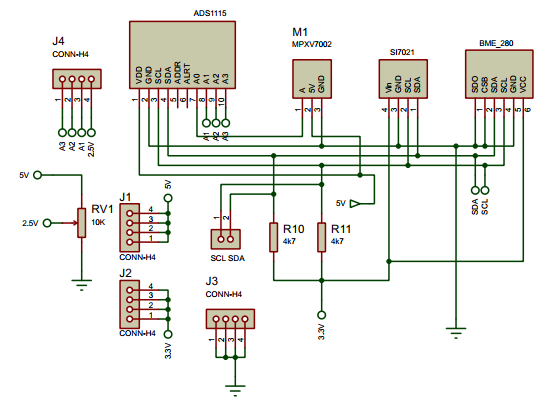
\includegraphics[scale=1]{A_Placa_5.png}
	\captionof{figure}{Esquema de sensores}
\end{figure}


\newpage




\begin{center}
		{
\includegraphics[width=0.2\textwidth]{unpsjb.png}\par}
	\vspace{1cm}
	{\bfseries\LARGE Universidad Nacional de la Patagonia\\ San Juan Bosco \par}
	\vspace{1cm}
	{\scshape\Large Facultad de Ingenier\'ia \par}
	\vspace{3cm}
	{\scshape\Huge Automatización de Túnel de Viento \par}
		{\itshape\Large -MANUAL DE USUARIO DE LA APLICACIÓN- \par}
	
	
	\vspace{3cm}
	{\itshape\Large Proyecto Final de Carrera\\ - Ingeniería Electrónica - \par}
	\vfill
	{\Large Autores: \par}
	{\Large Caamiña Quineros, Daniela Beatriz\\ Yapura, Cristian Alejandro \par}
	\vfill
	{\Large Diciembre 2021 \par}
\end{center}





\newpage






\section{Manual de usuario de la aplicación}
\subsection{Descargas}
El siguiente proyecto con sus respectivos archivos se encuentra para ser descargado en el repositorio GitHub.
\begin{figure}[htb]
	\centering
	
\includegraphics[scale=0.5]{gitTunel.png}
	\captionof{figure}{Repositorio en Github}
	\label{fig:git}
\end{figure}

\url{https://github.com/UNPSJB-YC/Automatizacion_Tunel_UNPSJB}

\subsection{Requerimientos del sistema}
\begin{itemize}
	\item Windows preferentemente 64bits.
	\item Tener instalado driver de comunicación serial para CH340 (Se encuentra dentro del repositorio para su descarga) 
\end{itemize}


\subsection{Puesta en marcha}
\begin{enumerate}
	\item Alimente variador de velocidad y el motor.
	\item Coloque los parámetros \textit{F35} y \textit{F36} del variador de velocidad en \textit{"20"} (tiempo de aceleración y desaceleración).
	\item Coloque el parámetro \textit{F7} del variador en \textit{"1"} (Fuente de control de la operación, para que las entradas digitales sean quienes controlen el motor).
	\item Enchufe a 220V el cable de alimentación que sale de la caja de control.
	\item Conecte el cable USB.
	\item Ejecute el programa \textit{Gui\_Tunel.exe} que se encuentra dentro de la carpeta \textit{application.windows64} dentro de \textit{Aplicación}.
	\item Seleccione el puerto dónde se encuentra conectado el microcontrolador.
	\subitem El puerto puede ser observado en \textit{Administrador de dispositivos} $\rightarrow$ \textit{Puertos (COM y LPT)} en Windows.
	\item Active el puerto.
	\item Al inicializar el puerto, el microcontrolador comienza a entregar valores a la aplicación por lo que se observa THP, velocidad estimada y frecuencia de referencia. 
	
\end{enumerate}

\begin{figure}[H]
	\centering
	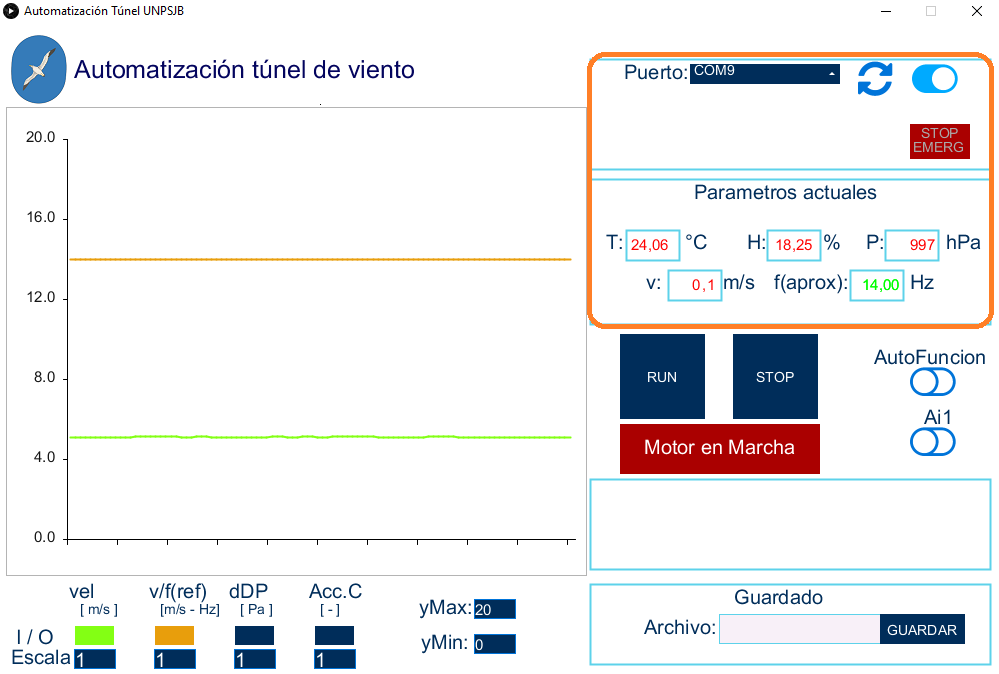
\includegraphics[scale=0.5]{capt2.png}
	\captionof{figure}{Puerto activado. Visualización de los valores del $\mu$C.}
	\label{fig:capt2}
\end{figure}



\subsection{Gráfico en tiempo real}
\subsubsection{Visibilidad de las señales en tiempo real}
En la parte izquierda inferior del programa, se puede activar o desactivar la visibilidad de las variables a observar, solo basta realizar un click en los rectángulos, y estos al estar activados se colocarán del color correspondiente a la señal.

\subsubsection{Escala}
En la parte inferior se encontrará “Escala” donde se establece la escala correspondiente de cada señal.
\begin{enumerate}
	\item Realice click en el interior del rectángulo
	\item Borre el número que posee y coloque el valor nuevo a ingresar.
	\item Presione “enter”.
	\item La escala de la señal elegida será modificada.
	
\end{enumerate}

\textbf{Ejemplo de escala:}

Si se coloca en una señal “escala: 10”, la variable observada en tiempo real estará aumentada 10 veces.

\subsubsection{Límite del eje vertical}
El eje vertical del gráfico en tiempo real puede ser modificado según necesidad.

\begin{enumerate}
	\item Realice click en el interior del rectángulo.
	\item Borre el número que posee y coloque el valor nuevo a ingresar.
	\item Presione “enter”.
	\item El eje “vertical” se verá modificado.
	
\end{enumerate}


\begin{figure}[H]
	\centering
	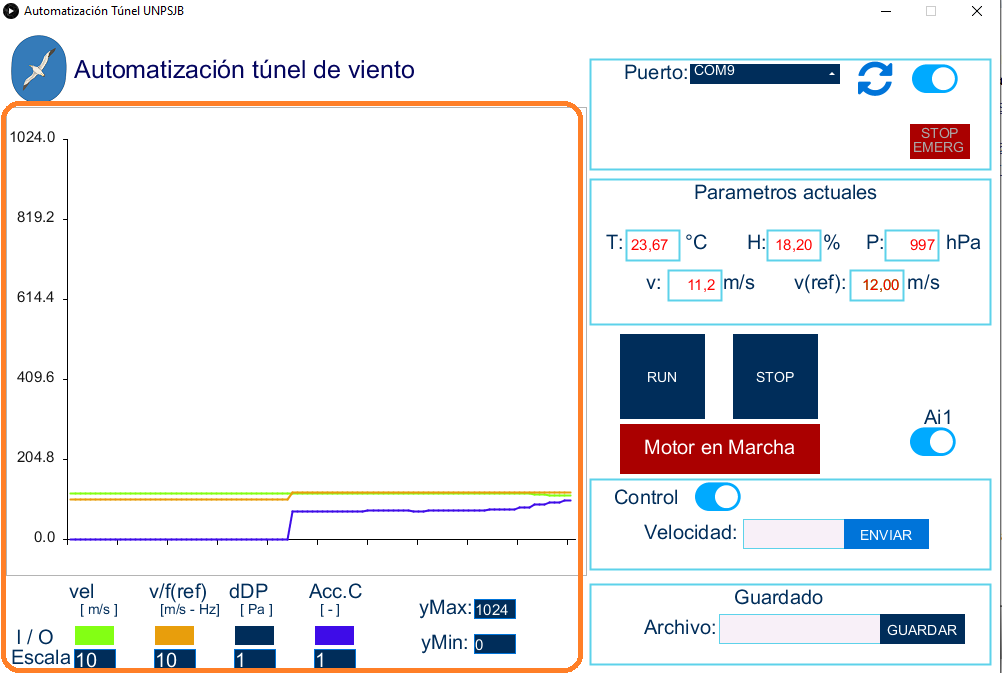
\includegraphics[scale=0.5]{capt3.png}
	\captionof{figure}{Gráfico en tiempo real}
	\label{fig:capt3}
\end{figure}

\subsection{AutoFuncion}
El modo de AutoFuncion carga un archivo “.csv” que se encuentra dentro de la carpeta “autofun” (Figura \ref{fig:autof2}). El archivo “.csv” posee los datos pertenecientes a los escalones de velocidad deseados y el tiempo de ejecución de cada uno (Figura \ref{fig:autof22}).

\begin{figure}[H]
	\centering
	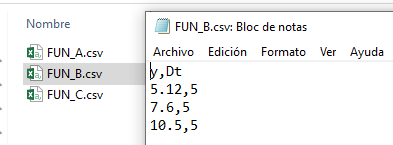
\includegraphics[scale=0.7]{carpcsv.png}
	\captionof{figure}{Archivos dentro de la carpeta "{}autofun"}
	\label{fig:autof2}
\end{figure}

\begin{figure}[H]
	\centering
	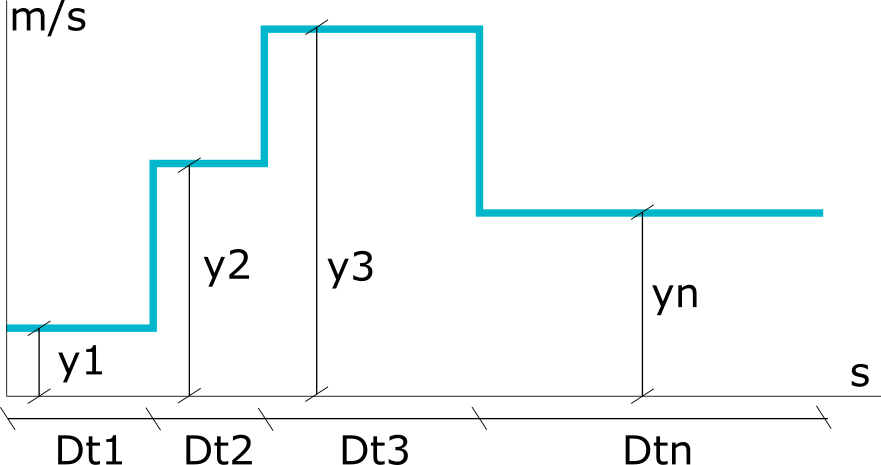
\includegraphics[scale=0.3]{autofej.png}
	\captionof{figure}{Diagrama para el formato de autofunción}
	\label{fig:autof22}
\end{figure}

El archivo debe ser generado por el usuario en un bloc de notas, guardado como formato  ``.csv'' y tener el formato observado en la Tabla \ref{tab:formcsv}, donde se ve que posee un encabezado el cual debe incluirse y las columnas son separadas por \textit{comas}. La primer columna, valores de velocidad en $m/s$, deben ser números comprendidos entre 4.7 y 18, los números decimales deben ser separados de la parte entera por medio de un punto. La segunda columna establece la cantidad de segundos de cada escalón preestablecido.
\begin{table}[h]
	\centering
	\begin{tabular}{|l|}
		\hline
		y,Dt \\ \hline
		y1,Dt1 \\ \hline
		y2,Dt2 \\ \hline
		y3,Dt3 \\ \hline
		...yn,Dtn \\ \hline
	\end{tabular}
	
	\caption{Formato para la confección del archivo .csv}
	\label{tab:formcsv}
\end{table}


Una vez que se eligió el archivo deseado del menú desplegable, se debe presionar el botón ``Abrir'' y aparecerá una señal visual debajo del mismo dando a conocer la implementación en el variador de dicha función (Figura \ref{fig:autof1}), el motor se pondrá en marcha y se apagará al finalizar la \textit{autofunción}.\\
Este sistema de datos puede tener hasta 6 valores de velocidad preestablecidos.

\begin{figure}[htb]
	\centering
	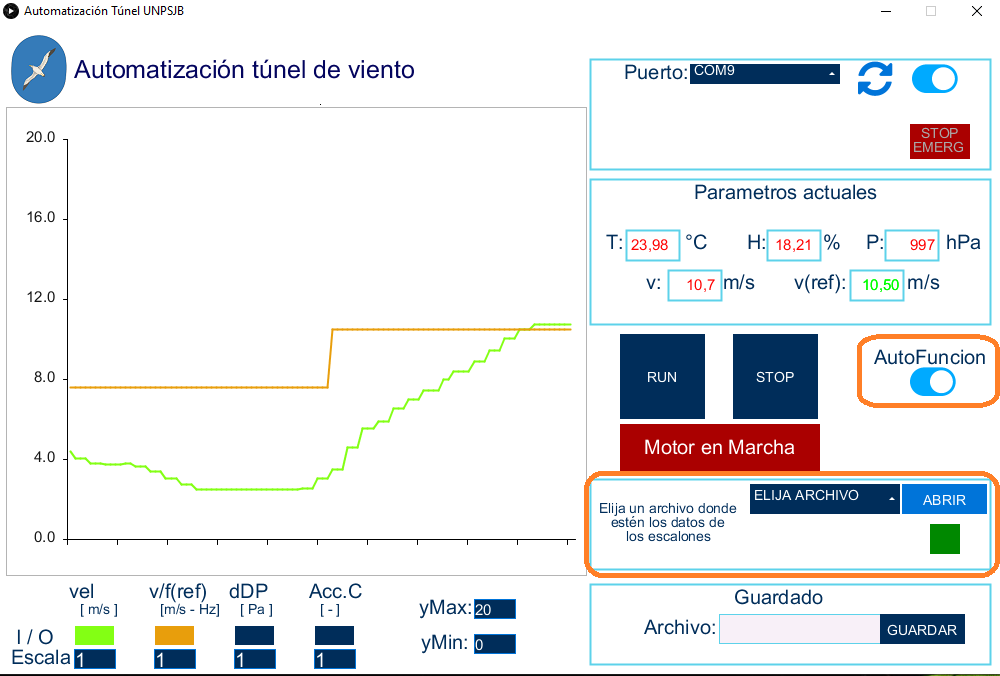
\includegraphics[scale=0.5]{capt1.png}
	\captionof{figure}{Aplicación en modo AutoFuncion}
	\label{fig:autof1}
\end{figure}





\subsection{Ai1}
\subsubsection{Control desactivado}
Al utilizar este modo de funcionamiento, se puede ingresar el valor deseado de frecuencia de salida del variador. El lazo de control estará abierto.

\subsubsection{Control activado}
El lazo de control estará activado, ante perturbaciones el sistema tiende a establecerse a la velocidad estipulada. Para determinar la velocidad de referencia se debe presionar sobre la caja de “velocidad”, ingresar un valor y presionar sobre el botón “enviar”.

\subsection{Encendido/ apagado del motor}
El encendido/ apagado del motor se puede realizar de dos formas:
\subsubsection{Panel frontal}
Si el parámetro F7 del variado de velocidad se encuentra en “0”, la marcha y parada del motor será realizada por los botones físicos en el panel frontal del variador.
\subsubsection{Aplicación}
Si el parámetro F7 del variador se encuentra en “1”, la marcha y parada del motor será realizada por los botones propios de la aplicación.


\subsection{Guardado de datos}
Una vez que se establece la comunicación, el programa realiza la captura de datos, al colocar un nombre y presionar el botón guardar, se generará un archivo “.csv” con los datos que el microcontrolador capturó cada aproximadamente 55ms hasta ese momento. Estos archivos se guardarán en la carpeta "data1{}" dentro de la carpeta general de la aplicación. 

\textbf{\textit{Alerta:}} Una vez que se presiona el botón guardar o el puerto se cierra los datos son borrados y se comenzará una nueva tabla.

\begin{figure}[H]
	\centering
	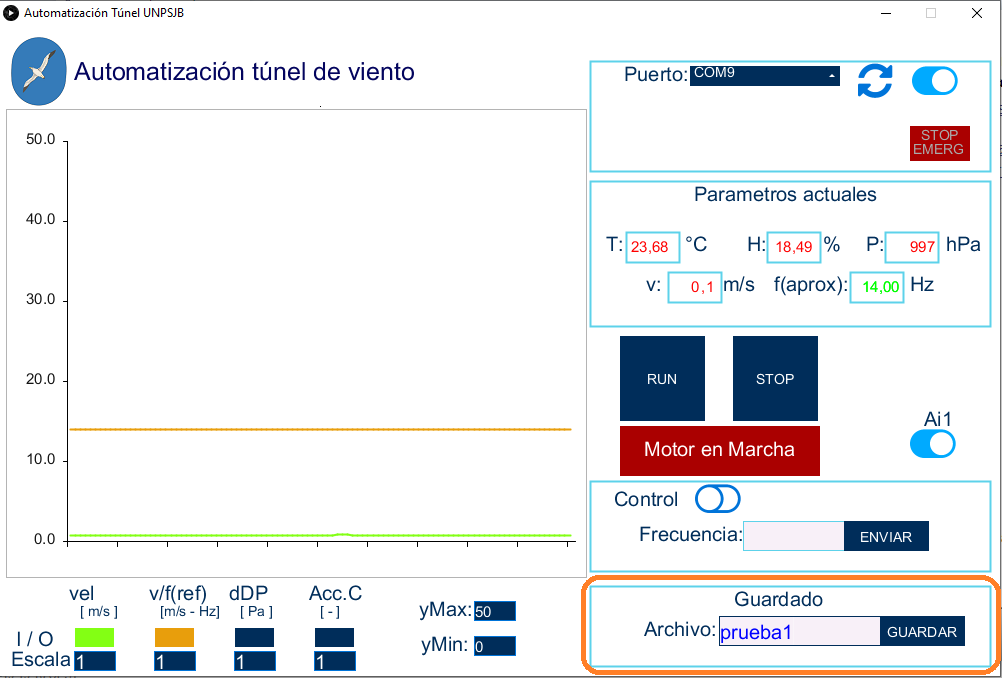
\includegraphics[scale=0.5]{capt4.png}
	\captionof{figure}{Guardado de datos}
	\label{fig:capt4}
\end{figure}


\subsection{Lectura de datos obtenidos}
El encabezado de la tabla (Figura \ref{fig:capt5}) muestra las siguientes leyendas:

\begin{itemize}
	\item \textit{Muestra:} número de muestra tomada
	\item \textit{Tiempo:} tiempo desde el inicio del puerto serie [ms].
	\item \textit{Temp:} temperatura ambiente [$^{\circ}$ C].
	\item \textit{Hum:} humedad relativa del ambiente [\%].
	\item \textit{Pres:} presión atmosférica [hPa].
	\item \textit{Den:} densidad estimada por el microcontrolador [$kg/m^3$].
	\item \textit{DP:} diferencia de presión medida a través del MPX7002 en conjunto con ADS1115 [Pa]
	\item \textit{Ref:} Valor de frecuencia o velocidad preestablecida [Hz ó m/s].
	\item \textit{VelFrec:} Velocidad del aire estimada [m/s].
	\item \textit{PWM:} señal de acción de control.
	\item \textit{Control:} señal de que el lazo de control está cerrado.
	\item \textit{Error:} error entre la velocidad estimada y la de referencia.
	\item \textit{ESTADOvariador:} estado encendido/apagado del motor.
	\item \textit{ERRORvariador:} indicación de algún error del variador de velocidad.
	\item \textit{TiempoRel:} indica tiempo desde el ultimo guardado de datos.
	\item \textit{ControlAutomatico:} indicación de comienzo y fin del control automático.
		
\end{itemize}
\begin{figure}[H]
	\centering
	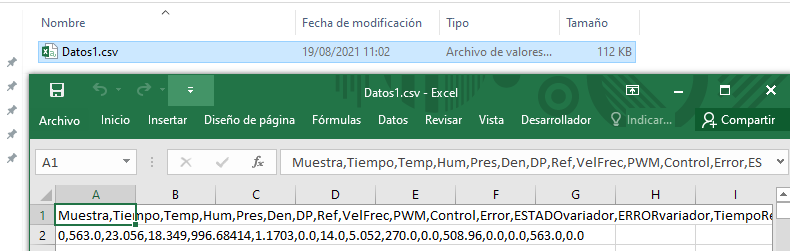
\includegraphics[scale=0.6]{capt5.png}
	\captionof{figure}{Archivo .csv generado}
	\label{fig:capt5}
\end{figure}
Para hacer lectura o interpretación de los datos se recomienda utilizar el script de Matlab \textit{Leer\_datos.m} (Figura \ref{fig:matlab1}) dentro de la carpeta dónde son guardados los archivos ("\textit{data1}"). El script está preparado para poder cambiar el nombre del archivo que se necesita leer y posee 3 ejemplos para observar el comportamiento.\\ En caso que el control esté apagado y se esté trabajando a lazo abierto, la línea punteada roja valdrá 0 y la velocidad de referencia será estimada.

\begin{figure}[H]
	\centering
	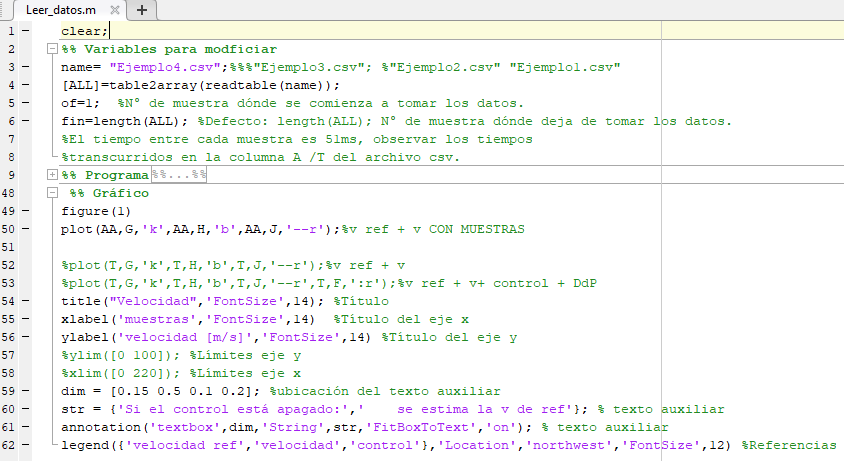
\includegraphics[scale=0.7]{matlab1.png}
	\captionof{figure}{Script de Matlab}
	\label{fig:matlab1}
\end{figure}

\begin{figure}[H]
	\centering
	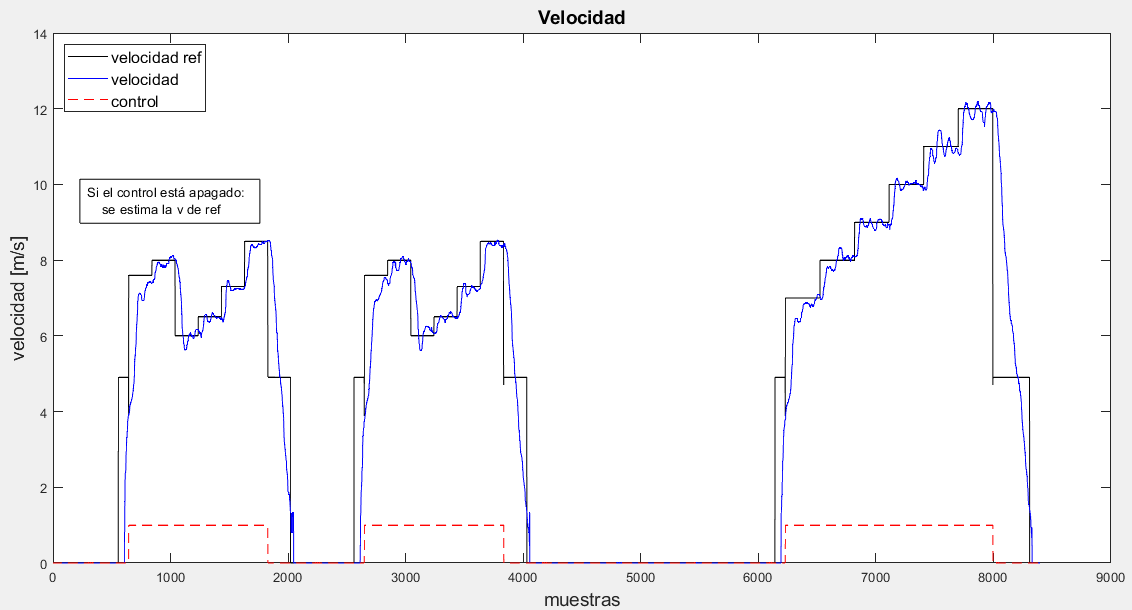
\includegraphics[scale=0.5]{matlab2.png}
	\captionof{figure}{Ejemplo del script}
	\label{fig:matlab2}
\end{figure}

\subsection{Falla externa}
	Al presionar el botón de “Falla externa” el $\mu$C enviará una señal al variador y el sistema se detendrá. Luego, se podrá restablecer al presionar el botón de \textit{reset}.

\newpage





